\documentclass[a4paper]{article}

\usepackage[english]{babel}
\usepackage[latin1]{inputenc}
\usepackage{amssymb}
\usepackage{framed}
\usepackage{graphicx}
\graphicspath{ {./img/} }

\usepackage{graphicx}
\usepackage{subcaption}
\usepackage{mwe}


\setlength{\parindent}{0pt}
\setlength{\parskip}{3ex}

\begin{document}

\begin{center}
  {\large Artificial Neural Networks and Deep Architectures, DD2437}\\
  \vspace{7mm}
  {\huge Short report on lab assignment 1\\[1ex]}
  {\Large Learning and generalisation in feed-forward networks ---\\[1ex]
 from perceptron learning to backprop}\\
  \vspace{8mm}  
  {\Large Ivan Stresec, Frano Rajic\\}
  \vspace{4mm}
  {\large September 9, 2020\\}
\end{center}

%\begin{framed}
%Please be aware of the constraints for this document. The main intention here is that you learn how to select and organise the most relevant information into a concise and coherent report. The upper limit for the number of pages is 6 with fonts and margins comparable to those in this template and no appendices are allowed. \\
%These short reports should be submitted to Canvas by the authors as a team before the lab presentation is made. To claim bonus points the authors should uploaded their short report a day before the bonus point deadline. The report can serve as a support for your lab presentation, though you may put emphasis on different aspects in your oral demonstration in the lab.
%Below you find some extra instructions in italics. Please remove them and use normal font for your text.
%\end{framed}

\section{Main objectives and scope of the assignment}

%\textit{List here a concise list of your major intended goals, what you planned to do and what you wanted to learn/what problems you were set to address or investigate, e.g.}\\
Our major goals in the assignment were  
\begin{itemize}
\item to recognize risks associated with backpropagation and minimize them for
robust learning of multi-layer perceptrons
\item to configure and monitor the behavior of learning algorithms for single- and
multi-layer perceptrons networks
\item to identify key limitations of single-layer networks
\item to design and apply networks in classification, function approximation and generalisation tasks
\end{itemize}

%\textit{Then you can write two or three sentences about the scope, limitations and assumptions made for the lab assignment}
% In this lab we implemented single- and multi-layer perceptrons with focus
% on the associated learning algorithms. Furthermore, we studied their properties by
% means of simulations.

In the first part of the lab, the focus was on two learning algorithms: the Delta rule for a
 single-layer perceptron and the generalized Delta rule for two-layer perceptron.
We used the created neural networks for classification, data compression, and function approximation.

In the second part of the lab assignment, we worked with multi-layer perceptrons to solve the problem of chaotic time series prediction. In this task we designed, trained, validated (including model selection) and evaluated the modeled neural
network with the ambition to deliver a robust solution with good generalization capabilities. % For this purpose, we exploited sckit-learn and TensorFlow libraries in Python.

\section{Methods}
%\textit{Mention here in just a couple of sentences what tools you have used, e.g. programming/scripting environment, toolboxes. If you use some unconventional method or introduce a clearly different performance measure, you can briefly mention or define it here.}\\
We have set up an Python 3.8 development environment in PyCharm IDE. Python libraries used include numpy, matplotlib, TensorFlow and scikit-learn. % We used GitHub to version the software.


\section{Results and discussion - Part I}

%\begin{framed}
%\textit{Make effort to be \textbf{concise and to the point} in your story of what you have done, what you have observed and demonstrated, and in your responses to specific questions in the assignment. You should skip less important details and explanations. In addition, you are requested to add a \textbf{discussion} about your interpretations/predictions or other thoughts concerned with specific tasks in the assignment. This can boil down to just a few bullet points or a couple of sentences for each section of your results. \\ Overall, structure each Results section as you like, e.g. in points. Analogously, feel free to group and combine answers to the questions, even between different experiments, e.g. with linearly separable and non-separable data, if it makes your story easier to convey. \\
%\\Plan your sections and consider making combined figures with subplots rather than a set of separate figures. \textbf{Figures} have to condense information, e.g. there is no point showing a separate plot for generated data and then for a decision boundary, this information can be contained in a single plot. Always carefully describe the axes, legends and add meaningful captions. Keep in mind that figures serve as a support for your description of the key findings (it is like storytelling but in technical format and academic style. \\
%\\Similarly, use \textbf{tables} to group relevant results for easier communication but focus on key aspects, do not overdo it. All figures and tables attached in your report must be accompanied by captions and referred to in the text, e.g. $"$in Fig.X or Table Y one can see ....$"$. \\
%\\When you report quantities such as errors or other performanc measures, round numbers to a reasonable number of decimal digits (usually 2 or 3 max). Apart from the estimated mean values, obtained as a result of averaging over multiple simulations, always include also \textbf{the second moment}, e.g. standard deviation (S.D.). The same applies to some selected plots where \textbf{error bars} would provide valuable information, especially where conclusive comparisons are drawn.} 
%\end{framed}

\subsection{Classification with a single-layer perceptron \textit{(ca.1 page)}}
%\textit{Combine results and findings from perceptron simulations on both linearly separable and non-separable datasets. Answer the questions, quantify the outcomes, discuss your interpretations and summarise key findings as conclusions.}

%Single layer perceptron - Perceptron learning rule (P.R.) and delta learning rule (D.R.). Through empirical ------something?(reasoning?)------ we came to all the following.
%The table with means and standard deviations of accuracy and convergence epochs can be seen in table \ref{TBD}.
%Note that the term convergence epoch is here used to describe the learning epoch in which the best solution was found and selected among others. The algorithm explored 50-150 more epochs than that to make see if a better solution can be found.
Perceptron learning rule (PR) converges faster for higher values of learning rate (ETA), as shown in table \ref{tab:pcn}. Delta learning rule (DR) converges faster for optimal learning rate. We have found that for batch learning the optimal is around 0.002 with 118 epochs, 100\% accuracy and MSE loss of 0.06. % Making the learning rate a bit higher like 0.003 makes the convergence faster: 3 as the average epochs and with accuracy of 100\%, but in the tradeoff for loss value which goes much higher with mean of 0.0?.
% On graphs in figure \ref{TBD} one can notice that the algorithm converges faster on 0.003 because the loss is only getting worse. % Furthermore, the values of loss that gets worse over epochs for learning rate 0.003 can be seen \ref{TBD}.
PR and DR both achieve accuracy of 100\% for separable dataset, but PR converges faster, as it takes more time for DR to minimize loss when the highest accuracy is already achieved.
As shown in tables \ref{tab:pcn_delta_batch} and \ref{tab:pcn_delta_seq}, both sequential and batch DR achieve accuracy of 100\%, but the effect of the learning rate is different. The optimal learning rate for batch is between 0.002 and 0.003, whereas the learning rate for sequential performs well on the whole range between 0.0001 and 0.2, but with much higher loss. % The loss comparison with respect to different learning rate values for sequential and batch learning can be seen on \ref{TBD}
The sequential converges faster than the batch DR. % In the general case where loss is preferred over convergence epochs, the sequential performs better aka converges faster than the batch D.R.
% The loss for the sequential D.R. is much more stochastic, as can be seen on figure \ref{TBD}.
The convergence speed is very sensitive on the initial weights for sequential learning, whereas for batch learning it is not very sensitive. % TODO check
D.R. with batch learning with no bias weights resulted in successful separation of classes if an separating line could be drawn through the origin of the coordinate system and in unsuccessful separation if it could not be drawn.

%	\label{tab:pcn}

% Please add the following required packages to your document preamble:
% \usepackage{graphicx}
\begin{table}[]
	\centering
	\caption{Perceptron learning rule}
	\label{tab:pcn}
	\resizebox{\textwidth}{!}{%
		\begin{tabular}{|l|r|r|r|r|r|r|r|}
			\hline
			Learning rate            & 0.001    & 0.005    & 0.01     & 0.1      & 0.25     & 1        & 10       \\ \hline
			Accuracy - mean          & 100.00\% & 100.00\% & 100.00\% & 100.00\% & 100.00\% & 100.00\% & 100.00\% \\ \hline
			Accuracy - std           & 0.00\%   & 0.00\%   & 0.00\%   & 0.00\%   & 0.00\%   & 0.00\%   & 0.00\%   \\ \hline
			Convergence epoch - mean & 29.22    & 8.26     & 3.45     & 1.91     & 1.90     & 1.93     & 1.87     \\ \hline
			Convergence epoch - std  & 27.84    & 6.80     & 2.14     & 0.38     & 0.30     & 0.32     & 0.42     \\ \hline
		\end{tabular}%
	}
\end{table}

% Please add the following required packages to your document preamble:
% \usepackage{graphicx}
\begin{table}[]
	\centering
	\caption{Batch delta learning rule}
	\label{tab:pcn_delta_batch}
	\resizebox{\textwidth}{!}{%
		\begin{tabular}{|l|r|r|r|r|r|r|r|}
			\hline
			Learning rate            & 0.0001   & 0.001    & 0.002    & 0.003    & 0.004    & 0.005    & 0.01     \\ \hline
			Accuracy - mean          & 100.00\% & 100.00\% & 100.00\% & 100.00\% & 100.00\% & 100.00\% & 100.00\% \\ \hline
			Accuracy - std           & 0.00\%   & 0.00\%   & 0.00\%   & 0.00\%   & 0.00\%   & 0.00\%   & 0.00\%   \\ \hline
			Convergence epoch - mean & 1,081.97 & 110.99   & 117.69   & 2.10     & 1.92     & 1.91     & 2.07     \\ \hline
			Convergence epoch - std  & 245.30   & 25.02    & 16.39    & 0.66     & 0.42     & 0.45     & 0.51     \\ \hline
			MSE Loss - mean          & 0.06     & 0.06     & 0.06     & 8.21     & 18.40    & 33.53    & 975.81   \\ \hline
			MSE Loss - std           & 0.00     & 0.00     & 0.00     & 9.89     & 27.26    & 50.83    & 5,597.03 \\ \hline
		\end{tabular}%
	}
\end{table}

\begin{table}[]
	\centering
	\caption{Sequential delta learning rule}
	\label{tab:pcn_delta_seq}
	\resizebox{\textwidth}{!}{%
		\begin{tabular}{|l|l|l|l|l|l|l|l|}
			\hline
			Learning rate            & 0.00     & 0.00     & 0.00     & 0.00     & 0.00     & 0.01     & 0.01     \\ \hline
			Accuracy - mean          & 100.00\% & 100.00\% & 100.00\% & 100.00\% & 100.00\% & 100.00\% & 100.00\% \\ \hline
			Accuracy - std           & 0.00\%   & 0.00\%   & 0.00\%   & 0.00\%   & 0.00\%   & 0.00\%   & 0.00\%   \\ \hline
			Convergence epoch - mean & 80.00    & 40.73    & 45.93    & 43.78    & 42.24    & 42.13    & 42.67    \\ \hline
			Convergence epoch - std  & 40.99    & 27.37    & 30.77    & 31.40    & 35.73    & 31.52    & 30.20    \\ \hline
			MSE Loss - mean          & 0.00     & 0.00     & 0.00     & 0.00     & 0.00     & 0.00     & 0.00     \\ \hline
			MSE Loss - std           & 0.00     & 0.00     & 0.00     & 0.00     & 0.00     & 0.00     & 0.00     \\ \hline
		\end{tabular}%
	}
\end{table}

We used inseparable two class datasets to train batch learning with various ways of subsampling the data to see the resulting effect on performance and boundary line position. In context of uneven class representation, the line will be drawn in such a way that the more frequent class gets higher individual accuracy. In context of non-representative class distribution, we came across a case where one part of the non-representative class was entirely disregarded and falsely classified as the opposite class by the decision boundary.
% The resulting decision boundaries for 4 different subsamples of the dataset are shown in figure \ref{fig:inseparable_datasets_lines}.
In all subsampling cases, we noticed that the real accuracy on the original non-subsampled dataset for all subsampled dataset was lower, which means that both non-representative sample distribution and uneven class representation decrease the generalization capability of the trained model.

%\begin{figure}
%	\centering
%	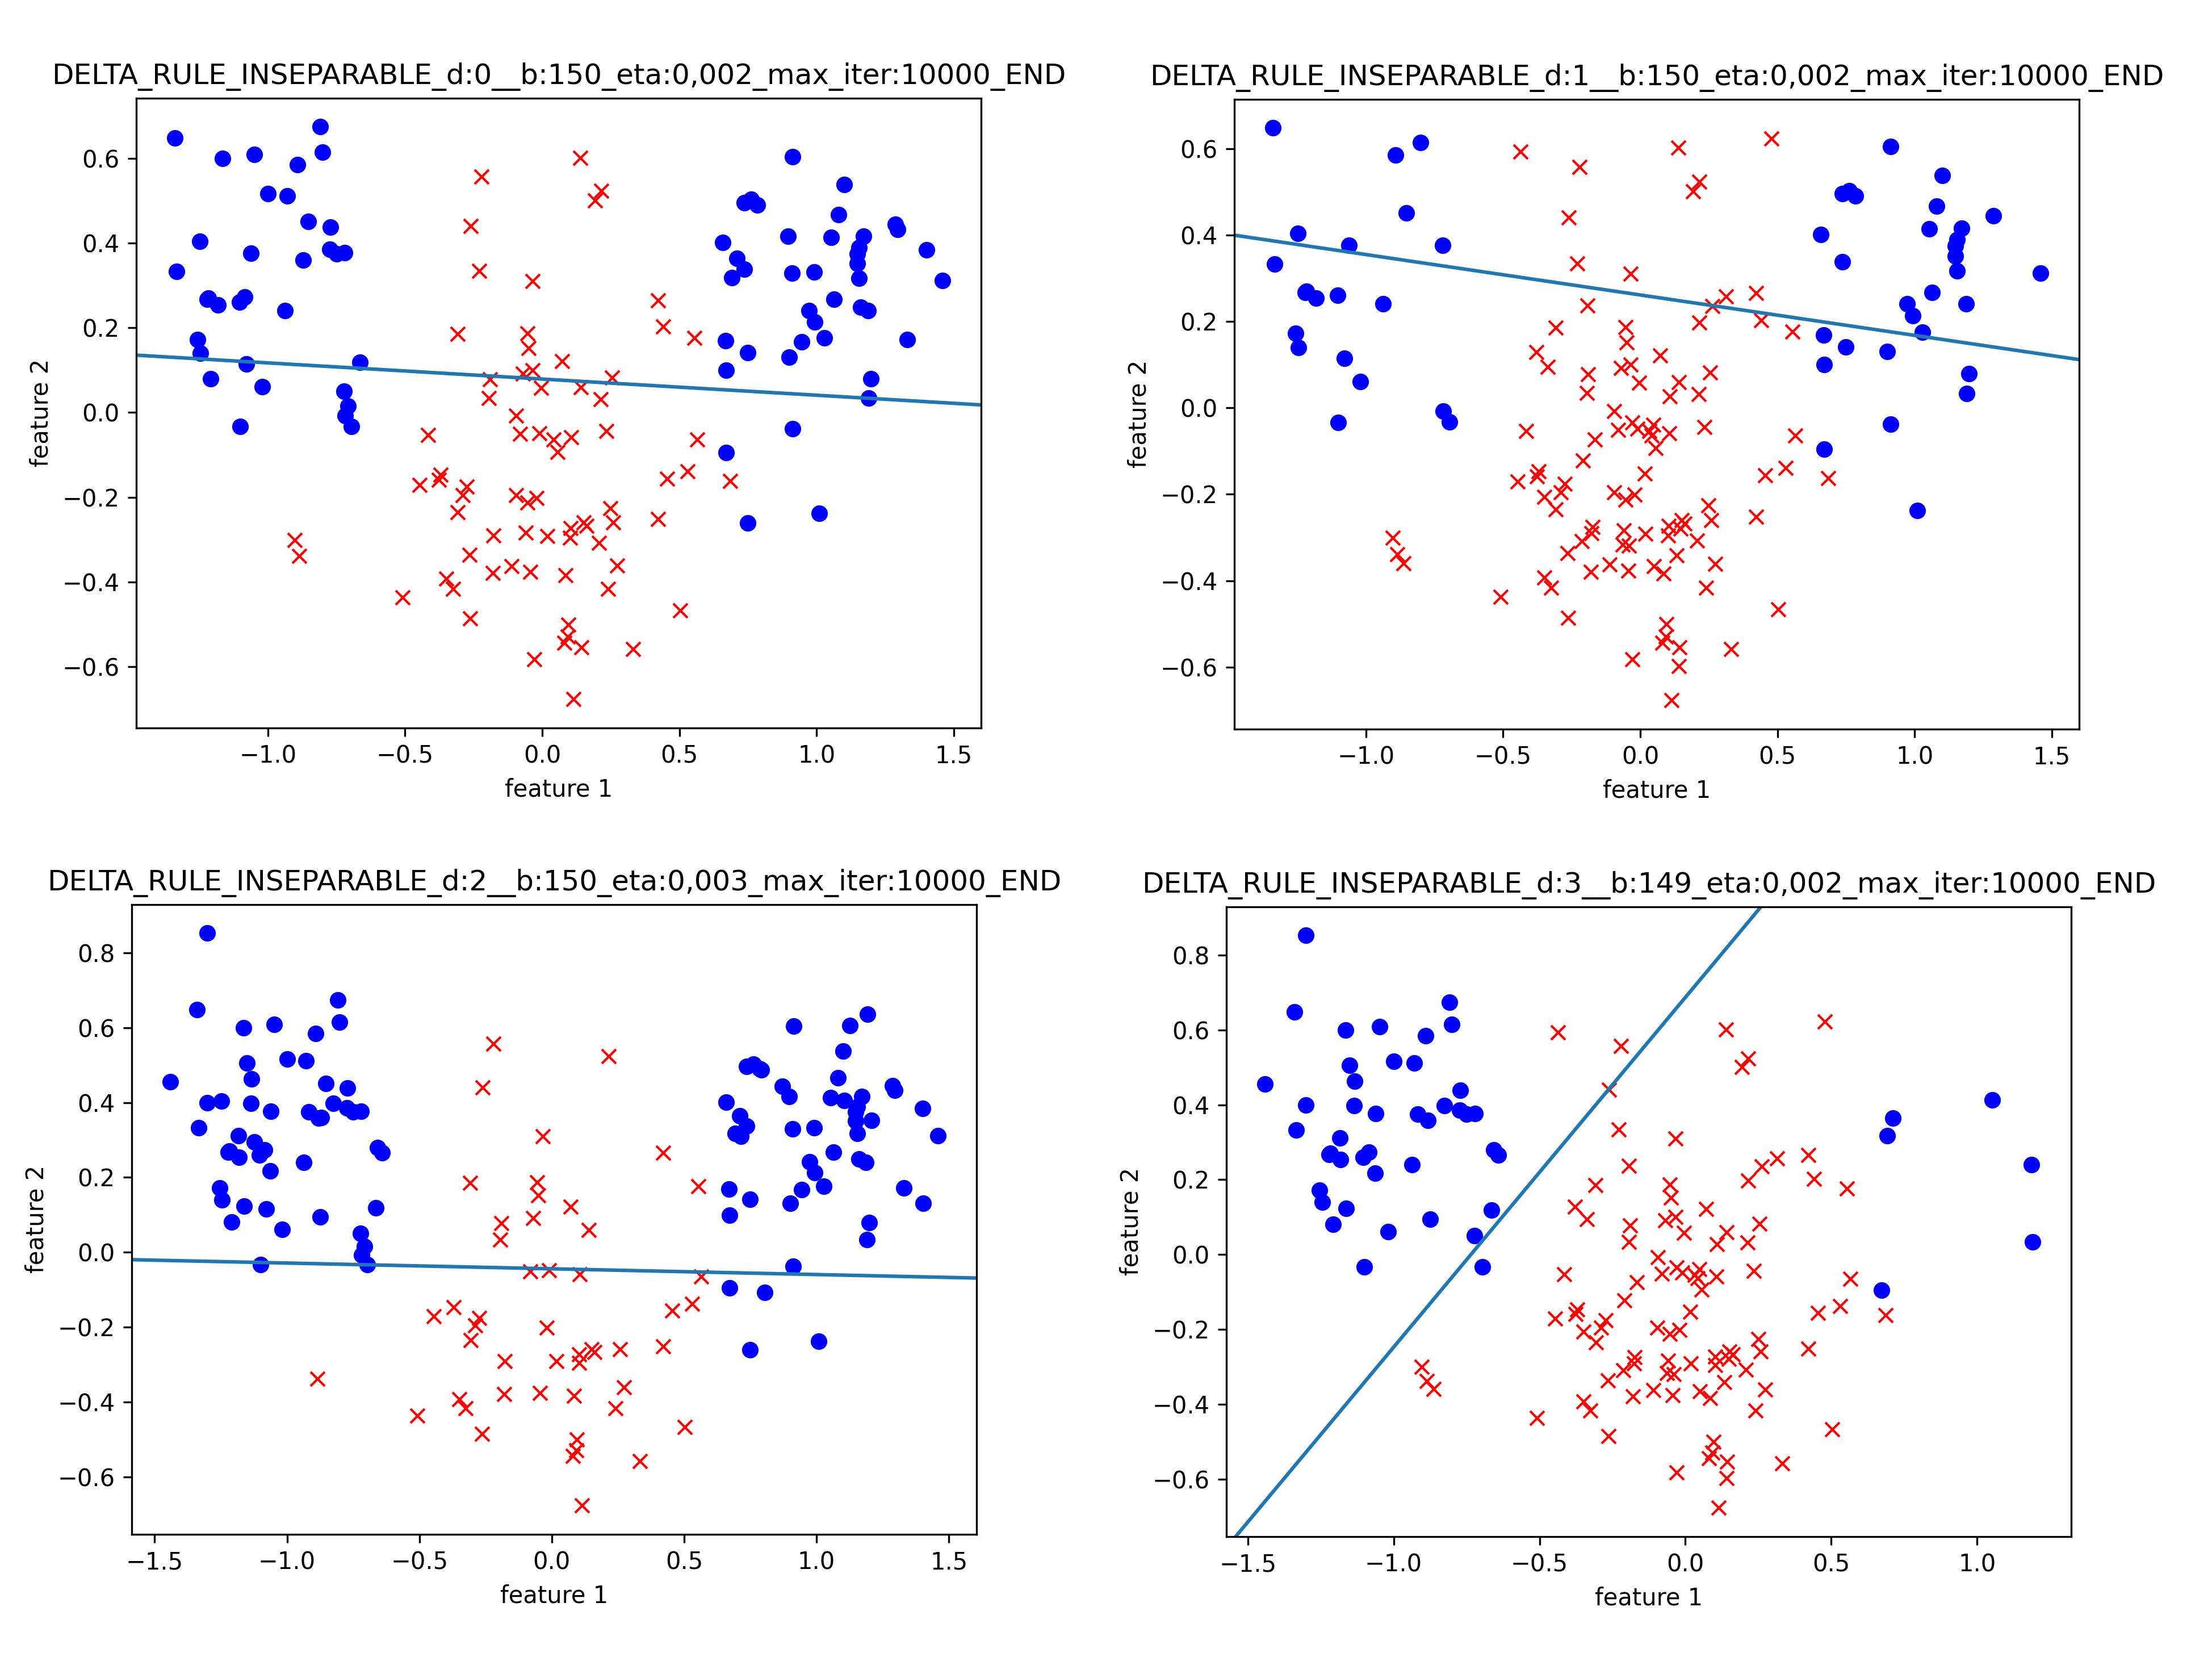
\includegraphics[width=10cm]{3.1.3_inseparable_datasets.png}
%	\caption{Decision boundaries for 4 subsampled datasets}
%	\label{fig:inseparable_datasets_lines}
%\end{figure}

In solving classification problem using an SLP one can easily observe its efficiency and its limitations.

Firstly, we have implemented the perceptron rule (implying a sequential learning scheme) and the Delta learning rule (batch learning) to a randomly generated, linearly separable classification dataset. Both have performed well and converged quickly...

Secondly, we have tested the differences between batch and sequential learning for the Delta rule SLP. In terms of epochs, both approaches converge relatively quickly, with ... being somewhat quicker

Thirdly, we have tested removing the bias term with the Delta rule in batch mode. Even without testing it, it is clear that the algorithm can converge only when the data is linearly separable by a line which goes through the center of the coordinate system. 



\subsection{Classification and regression with a two-layer perceptron \textit{(ca.2 pages)}}

\subsubsection{Classification of linearly non-separable data}
%\textit{It seems that one (decision boundary) or two plots (inclusing learning curves) should suffice. Build a story around the questions in the assignment. Include concise motivation for your findings and potential interpretations/speculations.}

\subsubsection{The encoder problem}
%\textit{Here you do not really need any illustrations, this could be a very short section reporting on your experiments in line with the assignment questions.}

\subsubsection{Function approximation}
%\textit{This subsection requires plots to reflect intuitive visual interpretation of the results. Make sure that you condense information and avoid any excessive plotting. Here you might also need to incorporate some illustration of the network's generalisation performance or use a table to systematically report the results requested in the assignment.}

\pagebreak
\section{Results and discussion - Part II \textit{(ca.2 pages)}}

%\textit{Here you do not have to introduce the problem or define Mackey-Glass time series, as you should focus on the results. You could divide them into two parts as the following two suggested subsections but you might as well keep your story under the main heading of Part II of the assignment. Importantly, always clearly state what network architecture you use, crucially with the number of hidden nodes, systematically report average results with various manipulations (regularisation etc.) and pay attention to differences between training, validation and test errors. Illustrating the outcome of your network predictions along with the original chaotic time series can also be very helpful. Finally, since you compare two- and three-layer architectures, make sure that you do not jump to any conclusions based on a small number of simulations unless you have statistically convincing evidence (when you comare the mean performance measures, their second moment is also relevant). In this part it may be particularly desirable to rely on tables.}

For this assignment, we have used the Mackey-Glass time series to evaluate a two-layer perceptron network. The data was simply generated by using the starting conditions and sequentially calculating values using the iterative formula given in the assignment. Furthermore, the data was split into three consecutive non-overlapping blocks for training, validation, and testing using 800, 200, and 200 values, respectively. For the regularisation method we have used weight decay with the L2 norm. Early stopping is implemented in such a way that if improvement (by at least $10^{-5}$) in the validation mean square error (MSE) is not visible for 50 iterations the learning stops. Also, the maximum number of epochs allowed is capped at 10000.

\subsection{Two-layer perceptron for time series prediction - model selection, regularisation and validation}
Using a rate of learning rate of 0.1 which showed good results and relatively fast convergence as well as a medium regularization coefficient $\lambda = 0.1$ several two-layer perceptrons were tested, the results of which we can see in table \ref{tab:learning_outcomes}. Each configuration was tested 10 times to calculate mean values and standard deviation. We opted for the networks with 8 nodes in the hidden layer as those show the best results on the test set.

\begin{table}[h!]
	\centering
	\begin{tabular}{|p{1.5cm}|p{2cm}|p{1.5cm}|}
		\hline
		nodes & MSE mean & MSE std\\
		\hline
		1 & 0.01413 & 0.01153 \\ \hline
		2 & 0.00916 & 0.00188 \\ \hline
		4 & 0.00870 & 0.00384 \\ \hline
		6 & 0.00806 & 0.00173 \\ \hline
		8 & 0.00774 & 0.00135 \\ \hline
	\end{tabular}
	\caption{Evaluation of various network configurations}
	\label{tab:learning_outcomes}
\end{table}

Furthermore, we have tested the impact of regularization strength on the selected network. Generally, one could expect that the weights of a network with stronger regularization tend to be closer to 0, but this effect was not obvious in our case, probably due to the fact that our networks are too simple to have problems with overfitting and larger weights. The described effect can to some extent be seen in figure \ref{fig:weight_histogram}.

\begin{figure}[h!]
	\begin{subfigure}{.5\linewidth}
		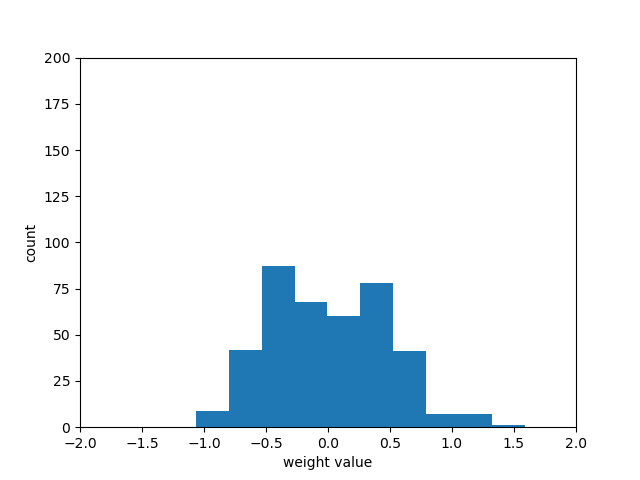
\includegraphics[width=165px]{images/weight_histogram_0.png}
		\centering
		\caption{\small No regularization}
	\end{subfigure}
	\begin{subfigure}{.5\linewidth}
		\centering
		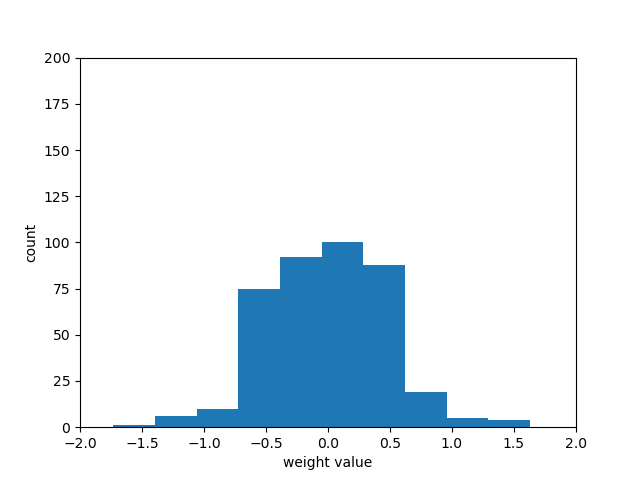
\includegraphics[width=165px]{images/weight_histogram_0_1.png}
		\caption{\small L2 regularization $\lambda = 0.1$}
	\end{subfigure}
	\caption{Weight distributions}
	\label{fig:weight_histogram}
\end{figure}

Finally, figure \ref{fig:learning_process} shows an example of the learning process and the outputs of our selected network with 8 nodes in the hidden layer, a learning rate of 0.1 and an L2 weight decay with $\lambda = 0.1$. The MSE on the test set of such a network can be seen in table \ref{tab:learning_outcomes}. The best of the 10 tested networks had an MSE of 0.00621 which demonstrates its good generalisation capabilities.

\begin{figure}[h!]
	\begin{subfigure}{.5\linewidth}
		
\includegraphics[width=165px]{images/learning_mse.png}
		\centering
		\caption{\small Learning process}
	\end{subfigure}
	\begin{subfigure}{.5\linewidth}
		\centering
		\includegraphics[width=165px]{images/predictions.png}
		\caption{\small Predictions after training}
	\end{subfigure}
	\caption{Weight distributions}
	\label{fig:learning_process}
\end{figure}

\subsection{Comparison of two- and three-layer perceptron for noisy time series prediction}

\section{Final remarks \normalsize{\textit{(max 0.5 page)}}}
% \textit{Please share your final reflections on the lab, its content and your own learning. Which parts of the lab assignment did you find confusing or not necessarily helping in understanding important concepts and which parts you have found interesting and relevant to your learning experience? \\
% Here you can also formulate your opinion, interpretation or speculation about some of the simulation outcomes. Please add any follow-up questions that you might have regarding the lab tasks and the results you have produced.}

\end{document}
